\documentclass[a4paper,12pt]{article}
\usepackage{amssymb}
\usepackage{amsmath}
\usepackage{amsthm} 
\usepackage{caption}
\usepackage{misccorr}
\usepackage[noadjust]{cite}
\usepackage{cmap} 
\usepackage[utf8]{inputenc}
\usepackage[T2A]{fontenc}
\usepackage[english, russian]{babel}
\usepackage{graphics}
\usepackage{graphicx}
\usepackage{textcomp}
\usepackage{verbatim}
\usepackage{makeidx}
\usepackage{geometry}
\usepackage{float}
\usepackage{bm}
\usepackage{esint}
\usepackage{mathtools}
\usepackage{graphicx}
\usepackage{listings}
\usepackage{courier}
\usepackage{multirow}
\usepackage{graphicx}

\lstset{basicstyle=\fontsize{10}{10}\selectfont,breaklines=true}

\newcommand{\specchapter}[1]{\chapter*{#1}\addcontentsline{toc}{chapter}{#1}}
\newcommand{\specsection}[1]{\section*{#1}\addcontentsline{toc}{section}{#1}}
\newcommand{\specsubsection}[1]{\subsection*{#1}\addcontentsline{toc}{subsection}{#1}}
\newcommand{\RNumb}[1]{\uppercase\expandafter{\romannumeral #1\relax}}
\newcommand{\jj}{\righthyphenmin=20 \justifying}


% геометрия
\geometry{pdftex, left = 2cm, right = 2cm, top = 2.5cm, bottom = 2.5cm}

\setcounter{tocdepth}{4} % фикс переноса 
\righthyphenmin = 2
\tolerance = 2048

\begin{document}
\thispagestyle{empty}

\noindent \begin{minipage}{0.15\textwidth}
	
\includegraphics[width=\linewidth]{b_logo}
\end{minipage}
\noindent\begin{minipage}{0.9\textwidth}\centering
	\textbf{Министерство науки и высшего образования Российской Федерации}\\
	\textbf{Федеральное государственное бюджетное образовательное учреждение высшего образования}\\
	\textbf{«Московский государственный технический университет имени Н.Э.~Баумана}\\
	\textbf{(национальный исследовательский университет)»}\\
	\textbf{(МГТУ им. Н.Э.~Баумана)}
\end{minipage}

\noindent\rule{18cm}{3pt}
\newline\newline
\noindent ФАКУЛЬТЕТ $\underline{\text{«Информатика и системы управления»}}$ \newline\newline
\noindent КАФЕДРА $\underline{\text{«Программное обеспечение ЭВМ и информационные технологии»}}$\newline\newline\newline\newline\newline\newline\newline


\begin{center}
	\noindent\begin{minipage}{1.3\textwidth}\centering
	\Large\textbf{  Лабораторная работа № 4}\newline
	\textbf{по дисциплине "Вычислительные алгоритмы"}\newline\newline\newline
	\end{minipage}
\end{center}

\noindent\textbf{Тема} $\underline{\text{Алгоритм наилучшего среднеквадратичного приближения.}}$\newline\newline
\noindent\textbf{Студент} $\underline{\text{Мицевич М. Д.}}$\newline\newline
\noindent\textbf{Группа} $\underline{\text{ИУ7-41Б}}$\newline\newline
\noindent\textbf{Оценка (баллы)} $\underline{\text{~~~~~~~~~~~~~~~~~~~~~~~~~~~}}$\newline\newline
\noindent\textbf{Преподаватель} $\underline{\text{Градов В.М.}}$\newline

\begin{center}
	\vfill
	Москва~---~\the\year
~г.
\end{center}
\clearpage

\section{Цель работы}

\noindent Получение навыков построения алгоритмаметода наименьших квадратовс использованием  полинома заданной  степени  при  аппроксимации табличных функций  с весами.

\section{Исходные данные}
\begin{enumerate}
    \item Таблица  функции  с весами $\rho_{i}$ и количеством  узлов N. Сформировать  таблицу самостоятельно со случайным разбросом точек. Предусмотреть  в  интерфейсе  удобную  возможность  изменения пользователем  весов  в таблице.
    \item Степень аппроксимирующего полинома - n.
\end{enumerate}

\section{Код программы}
\noindent\textbf{Листинг main.py:}
\lstinputlisting[frame=single, language=Python]{../main.py}

\noindent\textbf{\newline Листинг squares\_method.py:}
\lstinputlisting[frame=single, language=Python]{../squares_method.py}

\section{Результаты}

\subsection{Веса всех точек одинаковы}

\begin{center}
    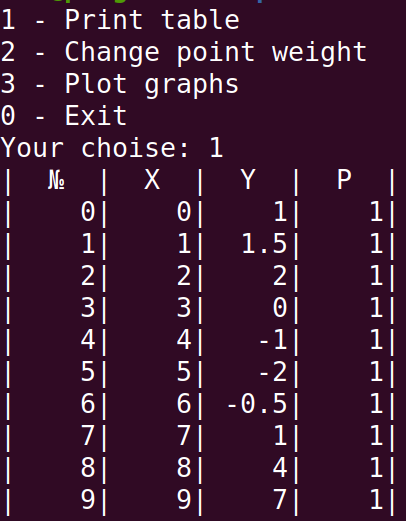
\includegraphics[width=6cm]{table1.png}
    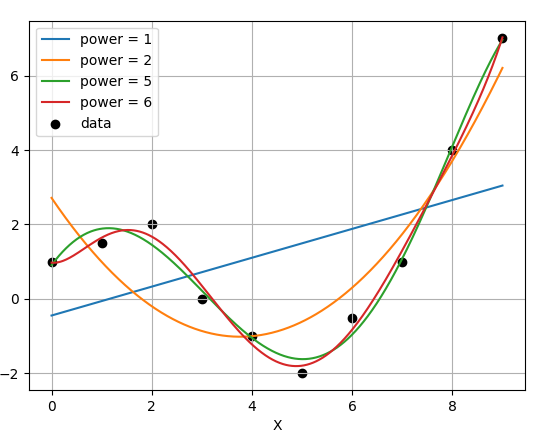
\includegraphics[scale=0.6]{graph1.png}   
\end{center}


\subsection{Веса точек разные}

\begin{center}
    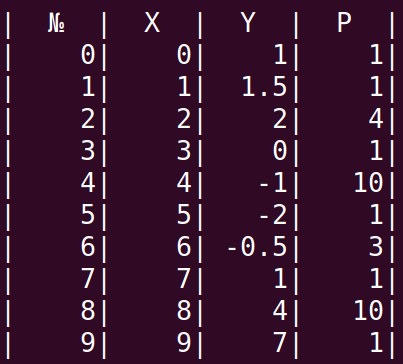
\includegraphics[width=6cm]{table2.png}
    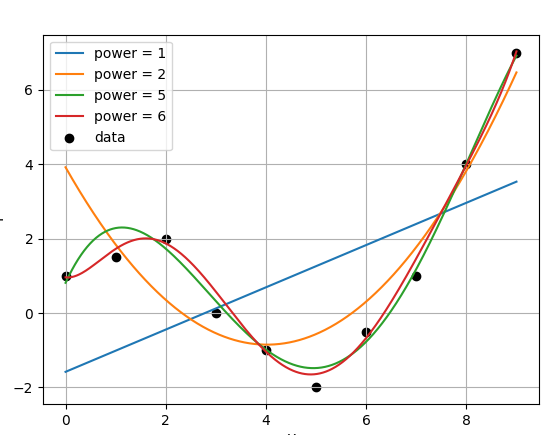
\includegraphics[scale=0.6]{graph2.png}   
\end{center}

\subsection{Изменение угла наклона прямой}

\begin{center}
    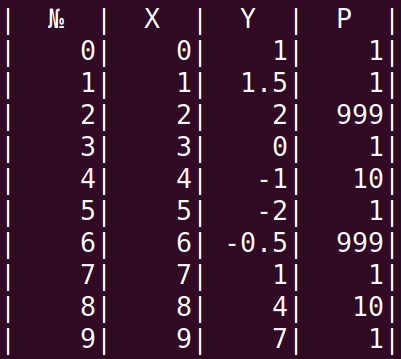
\includegraphics[width=6cm]{table3.png}
    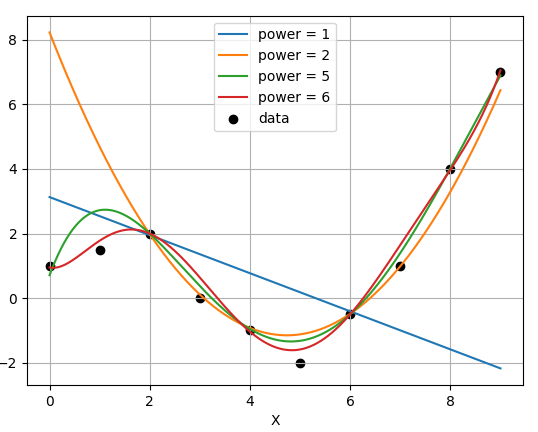
\includegraphics[scale=0.6]{graph3.png}   
\end{center}

\section{Контрольные вопросы}
\subsection{Что произойдет при задании  степени полинома n=N-1 (числу узлов таблицы минус 1)?}
График полинома пройдет через все точки вне зависимости от их веса

\subsection{Будет  ли  работать  Ваша  программа  при $n >= N$  Что  именно  в  алгоритме  требует отдельного анализа данного случая и может привести к аварийной остановке?}
Результат работы программы будет неверным. Аварийная ситуация может произойти при делении на ноль в решении СЛАУ

\subsection{Получить формулу для коэффициента  полинома $a_{0}$ при степени полинома n=0.Какой смысл имеет величина, которую представляет данный коэффициент?}

$a_{0} = \frac{\sum_{i=1}^{N} \rho_{i} * y_{i}}{\sum_{i=1}^{N} \rho_{i}}$

Данный коэффициент является взвешенным средним арифметическим ординат функции

\subsection{Записать и вычислить определитель матрицы СЛАУ для нахождения коэффициентов полинома для случая, когда n=N=2. Принять все $\rho_{i} = $1.}

$
\begin{vmatrix}
2 & x_1 + x_2 & x_1^2 + x_2^2 \\
x_1 + x_2 & x_1^2 + x_2^2 & x_1^3 + x_2^3 \\
x_1^2 + x_2^2 & x_1^3 + x_2^3 & x_1^4 + x_2^4
\end{vmatrix}
$
Определитель равен 0, поэтому система не имеет решения

\subsection{ Построить СЛАУ при выборочном задании степеней аргумента полинома $\phi(x) = a_0 + a_1 * x^m + a_2 * x^n$ причем степени n и m в этой формуле известны.}

$
\begin{cases}
    (x^0, x^0)*a_0 + (x^0, x^m)*a_1 + (x^0, x^n)*a_2 = (y, x^0) \\
    (x^m, x^0)*a_0 + (x^m, x^m)*a_1 + (x^m, x^n)*a_2 = (y, x^m) \\
    (x^n, x^0)*a_0 + (x^n, x^m)*a_1 + (x^n, x^n)*a_2 = (y, x^n)
\end{cases}
$

\subsection{Предложить схему алгоритма решения задачи из вопроса 5, если степени n и m подлежат определению наравне с коэффициентами $a_k$, т.е. количество неизвестных равно 5.}

Эту систему можно решить перебором всех допустимых значений n и m. Для каждой пары значений нужно найти коэффициенты и значение ошибки, после выбираем пару с наименьшей ошибкой.

\end{document}
